\documentclass[conference]{IEEEtran}
\IEEEoverridecommandlockouts

\usepackage{cite}
\usepackage{amsmath}
\usepackage{graphicx}
\usepackage{booktabs}
\usepackage{array}
\usepackage{multirow}
\usepackage{tikz}
\usetikzlibrary{arrows.meta,positioning,fit,backgrounds,calc}
\usepackage[hidelinks]{hyperref}
\usepackage{url}

\graphicspath{{../diagrams/}{../results/}}
\newcommand{\sig}[1]{\texttt{#1}}

\begin{document}

\title{Design and Evaluation of a Direct-Mapped Write-Back Cache Controller in Verilog}

\author{
\IEEEauthorblockN{Ashrith, Abhayanth K, Akhil, Srijan, Aryan Patel}
\IEEEauthorblockA{Modern Computer Architecture, Project 6\\
Source code: \url{https://github.com/Abhayanthk/direct-mapped-cache-controller}}
}

\maketitle

% ---------------------------------------------------------------------------
\begin{abstract}
A cache hides the latency of main memory by keeping recently used blocks in a small, fast store close to the processor. This paper presents the register-transfer-level design, verification and evaluation of a direct-mapped cache controller written in Verilog. The cache has 8 lines of 4-word (16-byte) blocks and sits between a processor testbench and a main-memory model that takes 4 clock cycles per word. An 8-bit word address is split into a 3-bit tag, a 3-bit index and a 2-bit offset. A five-state Mealy finite-state machine serves hits in one cycle, writes back a dirty block before refilling the line, and supports a write-back policy with a write-through mode selected by an input signal. Six test suites check every module and the integrated system against expected values. Four 64-access traces give hit rates of 75.0\% (sequential), 87.5\% (repeated), 28.1\% (random) and 0\% (conflicting), with an average memory access time (AMAT) between 3.62 and 22 cycles. Traffic measurements show that write-back reduces memory writes by 80\% for a workload that rewrites one word, but costs more traffic than write-through when each block is written only once or twice. The design synthesizes for a Lattice iCE40 HX8K FPGA using 28\% of the logic cells and closes timing at 82.87~MHz.
\end{abstract}

\begin{IEEEkeywords}
cache memory, direct-mapped cache, write-back, write-through, finite-state machine, Verilog, AMAT, FPGA
\end{IEEEkeywords}

% ---------------------------------------------------------------------------
\section{Introduction}

Processor speed has grown much faster than the speed of main memory, so a load or store that must reach DRAM can stall the processor for many cycles. Caches reduce this cost by exploiting \emph{temporal locality} (a recently used item is likely to be used again) and \emph{spatial locality} (items near a recently used item are likely to be used soon)~\cite{hennessy2019}. The design of a cache involves several choices: how blocks are mapped to lines, how large a block is, when main memory is updated on a write, and how the controller sequences the transfers between the cache and memory~\cite{smith1982}.

This project builds a complete, working cache at the register-transfer level so that each of these choices can be observed in simulation and measured. The goals were to:
\begin{enumerate}
\item implement a direct-mapped cache with tag, index and offset address decoding, a tag comparator and a controller finite-state machine (FSM);
\item support a write-back policy with dirty bits, plus a write-through mode for comparison;
\item verify every module and the integrated cache with self-checking testbenches;
\item measure hit rate, miss rate, AMAT and memory traffic on controlled access patterns; and
\item synthesize the design for a real FPGA to obtain its area and maximum clock frequency.
\end{enumerate}

Section~\ref{sec:lit} reviews related work. Section~\ref{sec:design} describes the proposed design. Section~\ref{sec:results} presents and discusses the results. Section~\ref{sec:contrib} lists the contribution of each team member, and Section~\ref{sec:concl} concludes.

% ---------------------------------------------------------------------------
\section{Literature Review}
\label{sec:lit}

\subsection{Origin and Organization of Caches}
Wilkes first proposed a small, fast ``slave'' memory that holds copies of words from a larger, slower main memory, which is the idea behind every modern cache~\cite{wilkes1965}. Smith's survey~\cite{smith1982} organized the design space that later work builds on: placement (direct-mapped, set-associative, fully associative), replacement, line (block) size, write policy and the effect of each on miss ratio and memory traffic. Standard textbooks~\cite{hennessy2019,patterson2017} express cache performance as the average memory access time,
\begin{equation}
\text{AMAT} = t_{\text{hit}} + m \cdot t_{\text{penalty}},
\label{eq:amat}
\end{equation}
where $m$ is the miss rate, and use the same equation to reason about the trade-offs below.

\subsection{Direct Mapping and Associativity}
In a direct-mapped cache each block can live in exactly one line, so a lookup needs one tag comparison and no replacement logic. Hill~\cite{hill1988} argued that this simplicity gives a shorter hit time, which can outweigh the higher miss rate of a set-associative cache. Hill and Smith~\cite{hillsmith1989} classified misses into \emph{compulsory}, \emph{capacity} and \emph{conflict} misses (the ``three Cs'') and quantified how associativity removes conflict misses. Jouppi~\cite{jouppi1990} showed that conflict misses are the main weakness of direct-mapped caches and reduced them with a small fully associative victim cache and with stream buffers that prefetch sequential blocks.

\subsection{Block Size}
A larger block brings neighbouring words in with each miss, which removes compulsory misses for code with spatial locality, but each miss then moves more data and takes longer. Przybylski, Horowitz and Hennessy~\cite{przybylski1988} studied these interactions between block size, cache size, associativity and memory timing, and showed that the best organization depends on the memory latency and transfer rate rather than on miss rate alone.

\subsection{Write Policies}
On a write hit, a write-through cache updates both the cache and main memory, while a write-back cache updates only the cache, marks the line dirty and writes the block to memory when it is evicted~\cite{smith1982}. Goodman~\cite{goodman1983} showed that caches can greatly reduce processor--memory bus traffic and proposed the write-once policy for shared-bus multiprocessors. Jouppi~\cite{jouppi1993} compared write-hit and write-miss policies in detail, including write-allocate (fetch-on-write) and no-allocate alternatives, and showed that the best choice depends on how often written data is written again before eviction.

\subsection{Hardware Implementation}
Patterson and Hennessy~\cite{patterson2017} describe a simple cache controller as a four-state FSM (idle, compare tag, write-back, allocate) for a write-back, write-allocate cache. Our controller follows this structure and adds a fifth state for write-through. The design is written in Verilog~\cite{ieee1364}, simulated with Icarus Verilog~\cite{icarus} and synthesized with the open-source Yosys and nextpnr flow~\cite{shah2019}.

\subsection{Position of This Work}
The works above analyse caches mostly through trace-driven simulation of large designs. This project instead builds a small cache at the register-transfer level, where the cost of each design decision is visible cycle by cycle: the dirty-block write-back before a refill, the extra memory accesses of a larger block, and the conflict misses of direct mapping. It measures the textbook quantities (hit rate, AMAT, write traffic) directly from hardware counters and checks them against a reference model.

% ---------------------------------------------------------------------------
\section{Proposed Solution}
\label{sec:design}

\begin{figure}[t]
\centering
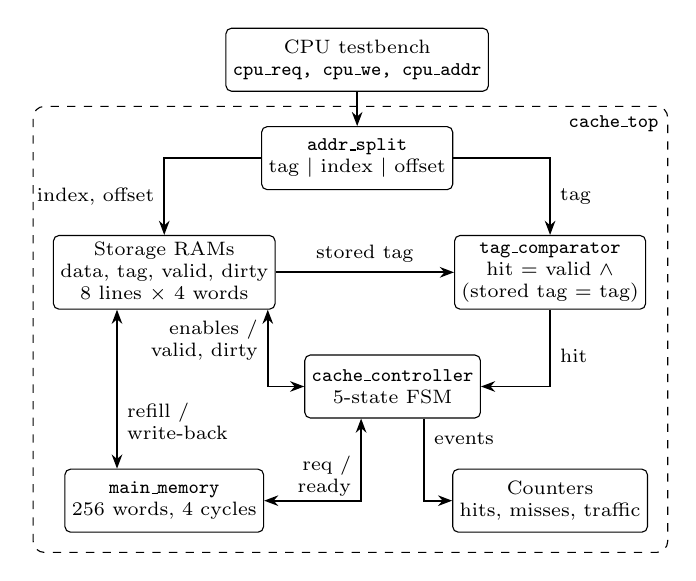
\begin{tikzpicture}[
  font=\scriptsize,
  box/.style={draw, rounded corners=2pt, align=center, minimum height=8mm, inner sep=2.5pt, fill=white},
  arr/.style={-{Stealth[length=1.8mm]}, semithick},
  darr/.style={{Stealth[length=1.8mm]}-{Stealth[length=1.8mm]}, semithick}]
\node[box] (cpu)   at (0, 0)      {CPU testbench\\\texttt{cpu\_req, cpu\_we, cpu\_addr}};
\node[box] (split) at (0, -1.25)  {\texttt{addr\_split}\\tag $|$ index $|$ offset};
\node[box] (rams)  at (-2.45, -2.7) {Storage RAMs\\data, tag, valid, dirty\\8 lines $\times$ 4 words};
\node[box] (cmp)   at (2.45, -2.7)  {\texttt{tag\_comparator}\\hit = valid $\wedge$\\(stored tag = tag)};
\node[box] (ctrl)  at (0.45, -4.15) {\texttt{cache\_controller}\\5-state FSM};
\node[box] (mem)   at (-2.45, -5.6) {\texttt{main\_memory}\\256 words, 4 cycles};
\node[box] (cnt)   at (2.45, -5.6)  {Counters\\hits, misses, traffic};

\draw[arr] (cpu) -- (split);
\draw[arr] (split.west) -| node[left, pos=0.75]{index, offset} (rams.north);
\draw[arr] (split.east) -| node[right, pos=0.75]{tag} (cmp.north);
\draw[arr] (rams.east) -- node[above]{stored tag} (cmp.west);
\draw[arr] (cmp.south) |- node[right, pos=0.3]{hit} (ctrl.east);
\draw[darr] (ctrl.west) -| node[left, pos=0.8, align=right]{enables /\\valid, dirty} ([xshift=-1mm]rams.south east);
\draw[darr] ([xshift=-6mm]rams.south) -- node[right, pos=0.7, align=left]{refill /\\write-back} ([xshift=-6mm]mem.north);
\draw[darr] ([xshift=-4mm]ctrl.south) |- node[left, pos=0.35, align=right]{req /\\ready} (mem.east);
\draw[arr] ([xshift=4mm]ctrl.south) |- node[right, pos=0.12]{events} (cnt.west);

\begin{scope}[on background layer]
\node[draw, dashed, rounded corners, fit=(split)(rams)(cmp)(ctrl)(mem)(cnt), inner sep=2.5mm] (top) {};
\end{scope}
\node[anchor=north east, font=\scriptsize\ttfamily] at (top.north east) {cache\_top};
\end{tikzpicture}

\caption{Block diagram of the cache system. The dashed box is the top module \sig{cache\_top}.}
\label{fig:arch}
\end{figure}

\begin{figure*}[t]
\centering
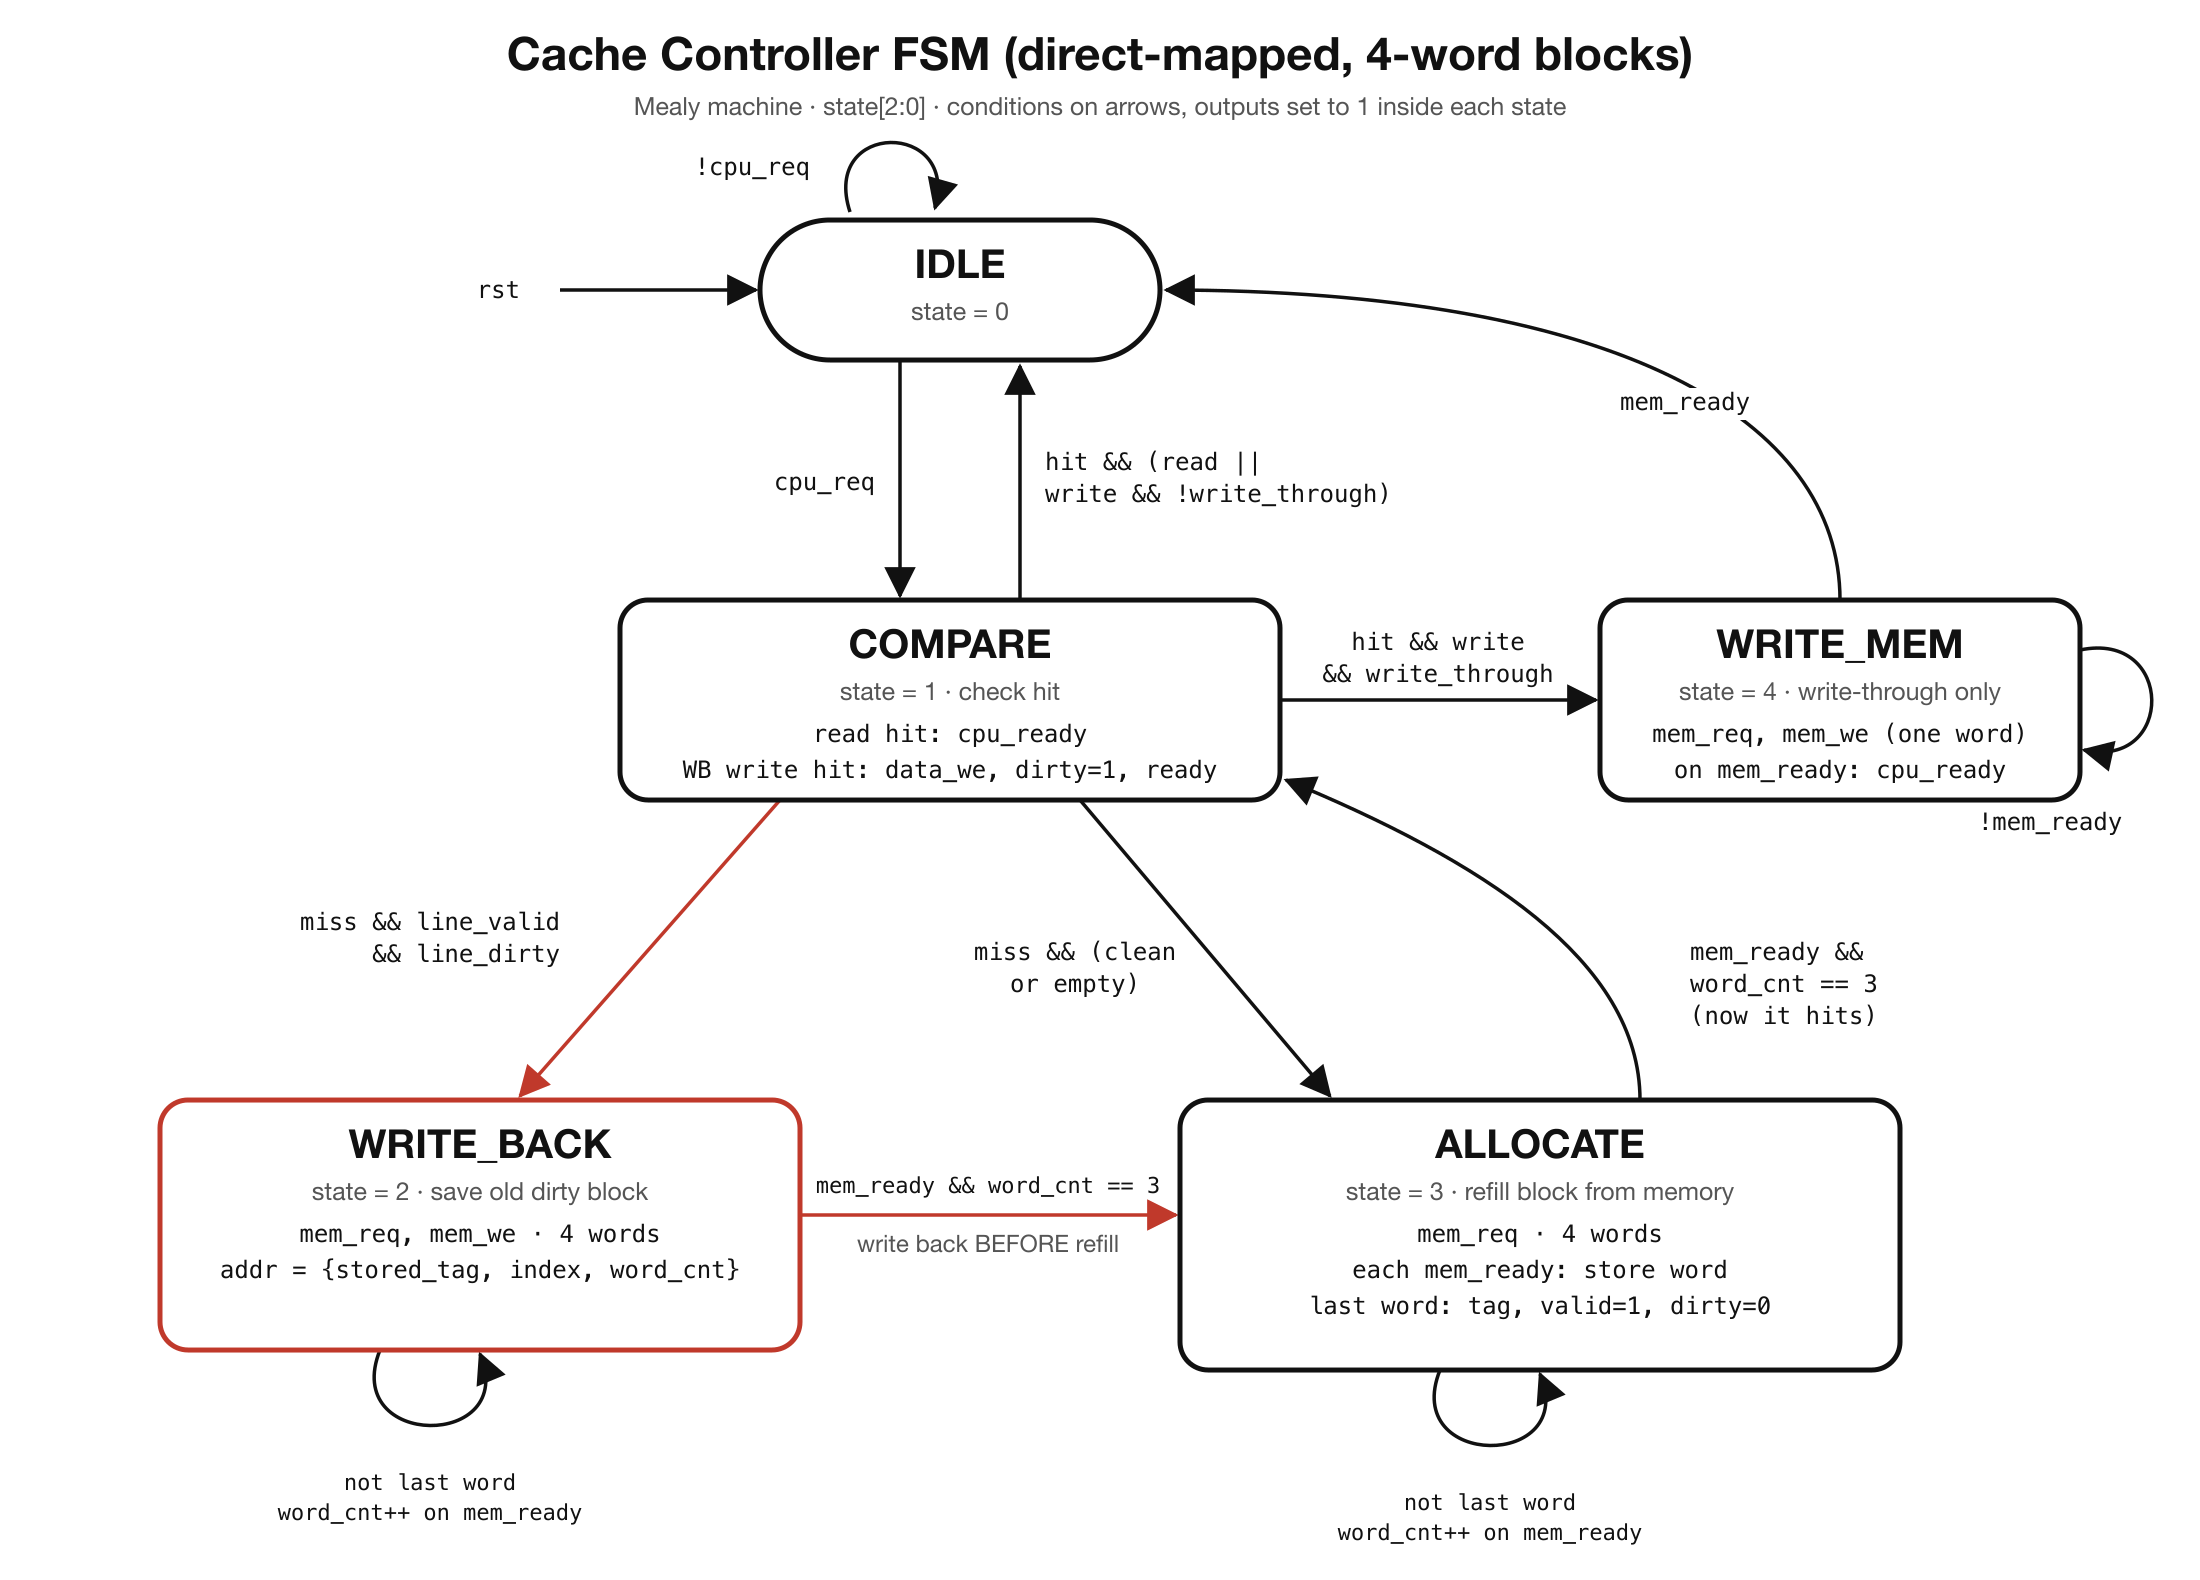
\includegraphics[width=0.72\textwidth]{fsm.png}
\caption{State diagram of the cache controller. Conditions are shown on the arrows and the outputs asserted in each state inside the boxes.}
\label{fig:fsm}
\end{figure*}

\subsection{System Overview}
Fig.~\ref{fig:arch} shows the system. The processor is a testbench that issues one request at a time with \sig{cpu\_req}, \sig{cpu\_we}, \sig{cpu\_addr} and \sig{cpu\_wdata}, and waits for \sig{cpu\_ready}. The top module \sig{cache\_top} connects the address splitter, the four storage arrays, the tag comparator, the controller, the main memory and the performance counters. Table~\ref{tab:params} lists the main parameters.


\begin{table}[t]
\caption{Cache Parameters}
\label{tab:params}
\centering
\footnotesize
\begin{tabular}{@{}ll@{}}
\toprule
Parameter & Value \\
\midrule
Main memory & 256 $\times$ 32-bit words (1~KB), 4 cycles/word \\
Organization & direct-mapped, 8 lines \\
Block size & 4 words (16 bytes) \\
Cache data & 128 bytes \\
Address split & tag [7:5], index [4:2], offset [1:0] \\
Bits per line & valid 1 + dirty 1 + tag 3 + data 128 = 133 \\
Write hit & write-back (default) or write-through \\
Write miss & write-allocate \\
Hit / clean miss / dirty miss & 1 / 22 / 42 cycles \\
\bottomrule
\end{tabular}
\end{table}

\subsection{Address Decoding and Hit Detection}
The module \sig{addr\_split} cuts the 8-bit word address into three fields. The index (bits 4:2) selects one of the 8 lines, the offset (bits 1:0) selects one of the 4 words in the block, and the tag (bits 7:5) identifies which of the 8 memory blocks that map to the line is present. For example, address 21 (\texttt{000\,101\,01}) is word~1 of the block held in line~5 with tag~0. The \sig{tag\_comparator} asserts \sig{hit} when the line's valid bit is set and the stored tag equals the address tag.

\subsection{Storage}
Each line has a valid bit, a dirty bit, a 3-bit tag and four 32-bit data words, stored in four arrays (\sig{data\_ram}, \sig{tag\_ram}, \sig{valid\_ram}, \sig{dirty\_ram}). Reads are combinational so that the lookup and the hit decision complete in the same cycle; writes happen on the rising clock edge. Valid and dirty bits are cleared on reset, so the cache starts empty.

\subsection{Main Memory Model}
The module \sig{main\_memory} models a slow DRAM with 256 32-bit words. After reset, word $a$ holds $\texttt{0x1000} + a$, which makes values easy to recognise in waveforms. The cache and the memory use a request/ready handshake: the controller raises \sig{mem\_req} (with \sig{mem\_we}, \sig{mem\_addr} and \sig{mem\_wdata}) and holds it, a synchronous counter \sig{wait\_count} counts 0 to 3, and on the fourth cycle the memory performs the read or write and raises \sig{mem\_ready} for exactly one cycle. Because neither side assumes how long the other takes, the latency can be changed without changing the controller. Every access also prints a log line, which makes memory traffic visible in simulation.

\subsection{Controller FSM}
The controller (Fig.~\ref{fig:fsm}) is a Mealy machine with five states:
\begin{itemize}
\item \textbf{IDLE} waits for \sig{cpu\_req}.
\item \textbf{COMPARE} checks for a hit. A read hit, or a write hit in write-back mode, finishes in this cycle; a write-back write hit also sets the dirty bit. A write hit in write-through mode goes to WRITE\_MEM. A miss on a valid dirty line goes to WRITE\_BACK; a miss on a clean or empty line goes to ALLOCATE.
\item \textbf{WRITE\_BACK} writes the four words of the old block to memory at addresses $\{\text{stored tag}, \text{index}, \sig{word\_cnt}\}$.
\item \textbf{ALLOCATE} reads the four words of the new block and stores each one as it arrives. With the last word it writes the tag, sets valid and clears dirty, then returns to COMPARE, where the request now hits.
\item \textbf{WRITE\_MEM} (write-through only) writes the word to memory and then signals \sig{cpu\_ready}.
\end{itemize}
A 2-bit counter \sig{word\_cnt} steps through the words of a block, advancing on each \sig{mem\_ready} during WRITE\_BACK and ALLOCATE. The design keeps four invariants: WRITE\_BACK always precedes ALLOCATE, so a dirty block is never overwritten before it is saved; the tag, valid and dirty bits change only with the last word of a refill; a block move takes exactly four memory accesses; and only a write hit in write-back mode sets a dirty bit.


\subsection{Datapath Multiplexers}
Three multiplexers in \sig{cache\_top} complete the datapath. The \emph{word select} chooses \sig{word\_cnt} during a block move and the CPU offset otherwise. The \emph{data RAM input} takes memory data during a refill and CPU data on a write hit. The \emph{memory address} is $\{\text{stored tag}, \text{index}, \text{word}\}$ for a memory write, so that a dirty block is saved to the address it came from, and $\{\text{address tag}, \text{index}, \text{word}\}$ for a memory read.

\subsection{Timing}
A hit is served in COMPARE in 1 cycle. Each memory word costs 5 cycles (4 cycles of latency plus the ready cycle), so a refill of 4 words takes 20 cycles. A clean miss therefore takes 22 cycles (COMPARE, 20 cycles of ALLOCATE, COMPARE again), giving a miss penalty of 21 cycles. A dirty miss adds a 20-cycle write-back, for 42 cycles. With these values, \eqref{eq:amat} becomes $\text{AMAT} = 1 + 21m$ cycles.

\subsection{Performance Counters}
The \sig{hit\_miss\_counter} counts a miss when the controller is in COMPARE without a hit and counts a hit when a request finishes without having missed, so the second COMPARE after a refill is not counted twice. The \sig{traffic\_counter} counts finished memory reads and writes in words.

\subsection{Verification Method}
Each module has a self-checking unit testbench, and two system testbenches drive \sig{cache\_top}:
\begin{itemize}
\item \textbf{Unit tests} cover storage (reset, per-line and per-word writes), hit logic (address split, every tag bit, counters), main memory (initial contents, 4-cycle latency, one-cycle ready pulse, top address, back-to-back accesses) and the controller (every state and transition in both modes, 4-word block moves).
\item \textbf{System test} T1--T7 in both write modes: read miss, read hit, hit on the next word of a block, write hit with dirty bit, dirty eviction, read-back of the evicted value, write miss and reset.
\item \textbf{Trace test} runs four 64-read traces and checks every access, both counters and the measured AMAT against a reference direct-mapped model.
\item \textbf{Traffic test} runs four workloads in both write modes and records memory reads, writes and cycles.
\end{itemize}
All tests are run by one script (\texttt{scripts/run.sh}) with Icarus Verilog~\cite{icarus}.

% ---------------------------------------------------------------------------
\section{Results and Discussion}
\label{sec:results}

\subsection{Functional Verification}
All six suites pass: the storage, hit-logic, main-memory and controller unit tests, the system test in both write-back and write-through modes, and the trace test. Fig.~\ref{fig:mem} shows the memory handshake: \sig{wait\_count} counts 0 to 3, \sig{mem\_ready} is high for one cycle, and the read returns \texttt{0x1005} for address~5. Fig.~\ref{fig:evict} shows test T4, a dirty eviction. Line~0 holds a block written by the CPU (address 0 = \texttt{0x0000AAAA}, dirty). A read of address 32, which also maps to line~0, first writes the four old words to memory addresses 0--3 (state~2) and only then reads addresses 32--35 (state~3), after which the request completes with \texttt{0x00001020}.

\begin{figure}[t]
\centering
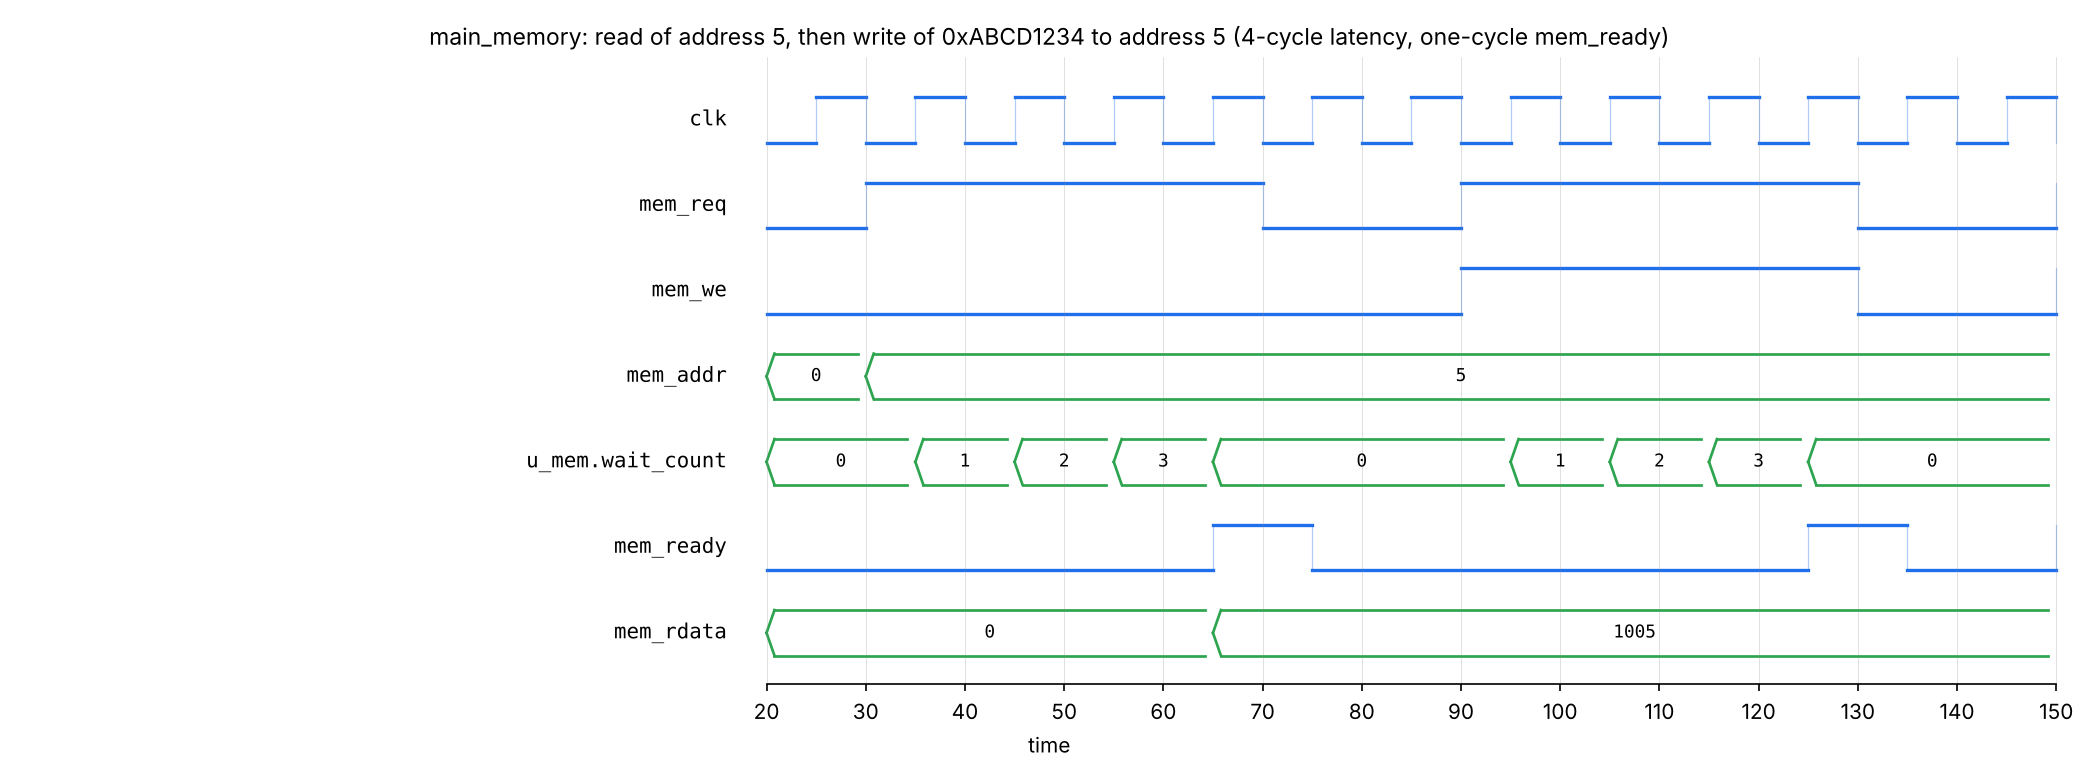
\includegraphics[width=\columnwidth]{member3-memory-wave.png}
\caption{Main-memory handshake: a read of address 5 followed by a write. Each access takes four counts of \sig{wait\_count} and ends with a one-cycle \sig{mem\_ready} pulse.}
\label{fig:mem}
\end{figure}

\begin{figure*}[t]
\centering
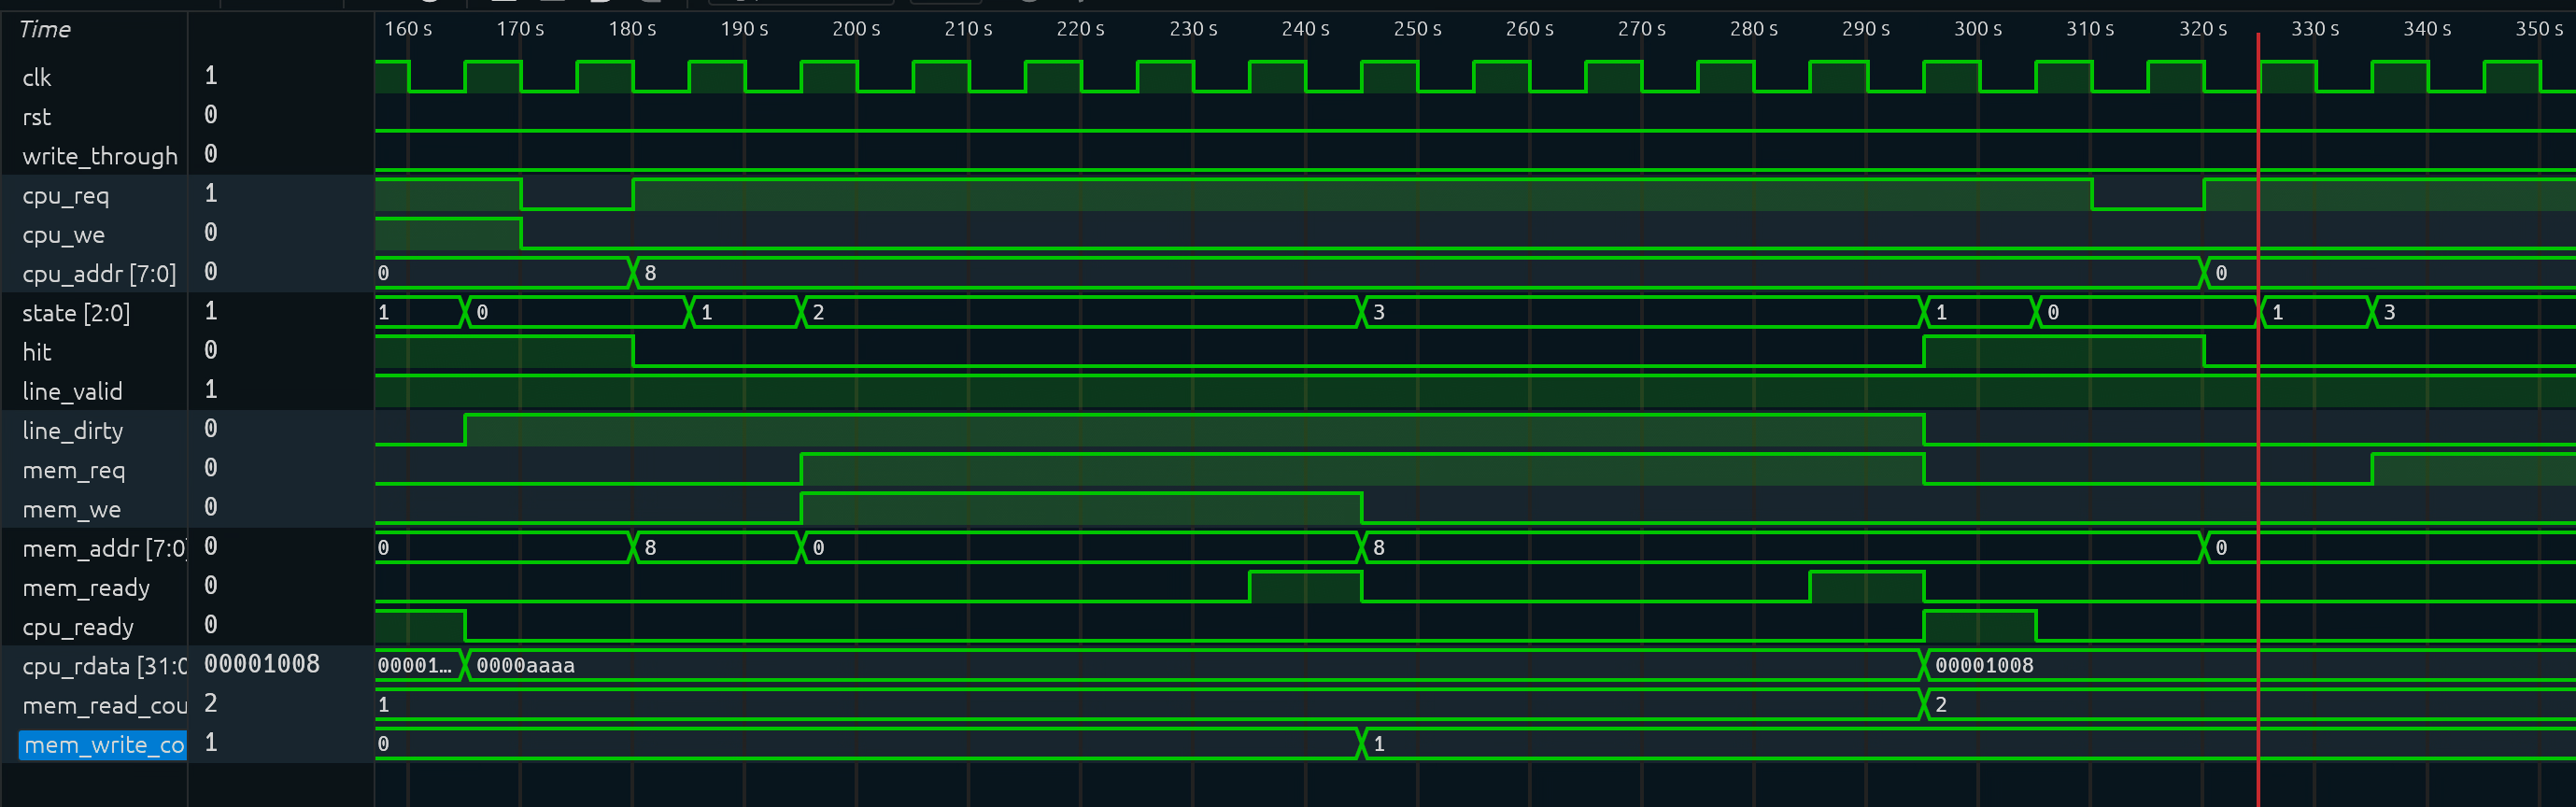
\includegraphics[width=\textwidth]{t4-dirty-eviction.png}
\caption{System test T4 (dirty eviction) in write-back mode. The controller enters WRITE\_BACK (state 2) and saves words 0--3 of the dirty block before ALLOCATE (state 3) reads words 32--35 of the new block.}
\label{fig:evict}
\end{figure*}

\subsection{Hit Rate and AMAT}
Table~\ref{tab:trace} gives the results of the four traces. The measured AMAT equals $1 + 21m$ for every trace.

\begin{table}[t]
\caption{Hit Rate and AMAT for Four 64-Read Traces}
\label{tab:trace}
\centering
\footnotesize
\begin{tabular}{@{}lrrrr@{}}
\toprule
Trace & Hits & Misses & Hit rate & AMAT (cycles) \\
\midrule
Sequential (0--63) & 48 & 16 & 75.0\% & 6.25 \\
Repeated (8 lines $\times$ 8) & 56 & 8 & 87.5\% & 3.62 \\
Random (0--127) & 18 & 46 & 28.1\% & 16.09 \\
Conflict (all line 0) & 0 & 64 & 0.0\% & 22.00 \\
\bottomrule
\end{tabular}
\end{table}

The traces isolate the three kinds of miss~\cite{hillsmith1989}:
\begin{itemize}
\item \textbf{Sequential} (spatial locality): the first read of each block misses and brings in all four words, so the next three reads hit. With 1-word blocks every access of this trace would miss, so the 4-word block raises the hit rate from 0\% to 75\%. The remaining misses are compulsory.
\item \textbf{Repeated} (temporal locality): addresses 0, 4, \dots, 28 use one line each and fit in the cache, so only the first of the eight passes misses.
\item \textbf{Random} (capacity): the trace covers 128 words, four times the 32 words the cache holds, so most blocks are evicted before reuse.
\item \textbf{Conflict}: address~1 alternates with 33, 65 and 129, which all map to line~0. Every access misses while the other seven lines stay empty. This is the weakness of direct mapping noted by Jouppi~\cite{jouppi1990}; a 2-way set-associative cache could keep address~1 in one way and hit on every return to it.
\end{itemize}

The block size also shows the trade-off described by Przybylski \emph{et al.}~\cite{przybylski1988}: 4-word blocks remove most compulsory misses on sequential code, but because memory moves one word per access, each miss costs 22 cycles instead of the 7 a 1-word block would need.

\subsection{Write-Back Versus Write-Through}
Table~\ref{tab:traffic} compares the two write policies on the same cache. Memory traffic is counted in words.

\begin{table}[t]
\caption{Memory Traffic of the Two Write Policies}
\label{tab:traffic}
\centering
\footnotesize
\begin{tabular}{@{}llrrr@{}}
\toprule
Workload & Policy & Reads & Writes & Cycles \\
\midrule
\multirow{2}{*}{W1: 20 writes to one word} & WB & 8 & \textbf{4} & \textbf{125} \\
 & WT & 8 & 20 & 205 \\
\midrule
\multirow{2}{*}{W2: 1 write in each line} & WB & 64 & 32 & 544 \\
 & WT & 64 & \textbf{8} & \textbf{424} \\
\midrule
\multirow{2}{*}{W3: read only} & WB & 32 & 0 & 216 \\
 & WT & 32 & 0 & 216 \\
\midrule
\multirow{2}{*}{W4: 2 writes in each line} & WB & 64 & 32 & 592 \\
 & WT & 64 & \textbf{16} & \textbf{512} \\
\bottomrule
\end{tabular}
\\[2pt]
\raggedright\scriptsize WB = write-back, WT = write-through. Each workload ends by evicting the written lines.
\end{table}

Write-back is clearly better when the same word is written many times (W1): it writes memory once per evicted block (4 words) instead of once per store, reducing memory writes by 80\% and total cycles by 39\%. This agrees with the traffic argument of Goodman~\cite{goodman1983}. When each line receives only one or two writes (W2, W4), write-through is better, because write-back saves the whole 4-word block on eviction while write-through sends only the words the processor wrote. Read-only code (W3) behaves identically under both policies. The result supports Jouppi's observation~\cite{jouppi1993} that the best write policy depends on how often data is rewritten before eviction. Per-word dirty bits (3 more bits per line) would let write-back save only the modified words and remove the penalty in W2 and W4.

\subsection{Synthesis}
The cache core (address split, storage, comparator and controller, without the memory model and the test counters) was synthesized with Yosys and placed and routed with nextpnr~\cite{shah2019} for a Lattice iCE40 HX8K. Table~\ref{tab:synth} summarizes the result.

\begin{table}[t]
\caption{Synthesis Results on the iCE40 HX8K}
\label{tab:synth}
\centering
\footnotesize
\begin{tabular}{@{}lr@{}}
\toprule
Resource & Used \\
\midrule
Logic cells & 2184 / 7680 (28\%) \\
LUT4 & 1132 \\
Flip-flops & 1071 \\
Block RAM & 0 / 32 \\
I/O pins & 153 / 206 (74\%) \\
Maximum frequency (target 50~MHz) & 82.87~MHz \\
\bottomrule
\end{tabular}
\end{table}

The flip-flop count matches the storage bits: 1024 data bits, 24 tag bits, 8 valid and 8 dirty bits, 3 state bits and 2 word-counter bits make 1069, and the tools add 2. The cache words use flip-flops rather than block RAM because the design reads the data array combinationally, while iCE40 block RAM reads only on a clock edge; most LUTs implement the 32-to-1 word multiplexer. The critical path, about 12~ns, runs from the tag RAM through the comparator and the COMPARE logic to the RAM write enables, since lookup and decision happen in the same cycle. At 82.87~MHz a hit takes 12.1~ns and a clean miss 265~ns.

\subsection{Limitations}
The design has one dirty bit per line, so a write-back always moves the whole block. Memory transfers one word per access with no burst mode, so a miss costs four full memory latencies. The cache is direct-mapped and handles one request at a time without a write buffer. The main memory is a fixed-latency model rather than a DRAM controller, and the FPGA design has been synthesized but not yet run on a board.

% ---------------------------------------------------------------------------
\section{Individual Contributions}
\label{sec:contrib}

The work was divided into five parts with fixed module and port names, so that each part could be built and unit-tested independently before integration. Each member committed their own work from their own account to the shared repository. Table~\ref{tab:contrib} summarizes the division.

\begin{table}[t]
\caption{Individual Contributions}
\label{tab:contrib}
\centering
\footnotesize
\begin{tabular}{@{}p{1.55cm}p{6.75cm}@{}}
\toprule
Member & Work \\
\midrule
Ashrith\newline\emph{Storage} & Data, tag, valid and dirty RAMs (\texttt{rtl/storage/}); storage unit test with additional per-line checks; storage waveform. \\
\addlinespace
Abhayanth K\newline\emph{Hit logic, analysis} & Repository structure; address splitter, tag comparator, traffic and hit/miss counters (\texttt{rtl/hit\_logic/}); hit-logic unit test; write-policy traffic test and comparison; extension to 4-word blocks with a word offset; access traces with hit-rate and AMAT checks; iCE40 synthesis flow; demonstration script; README; updated FSM diagram and waveforms. \\
\addlinespace
Akhil\newline\emph{Main memory} & Main-memory model with 4-cycle latency and request/ready handshake (\texttt{rtl/memory/}); main-memory unit test with added checks for the top address and back-to-back accesses; memory waveform. \\
\addlinespace
Srijan\newline\emph{Controller} & Controller FSM with compare, write-back, allocate and write-through states (\texttt{rtl/controller/}); controller unit test including empty-line and dirty write-miss cases; FSM diagram; controller waveform. \\
\addlinespace
Aryan Patel\newline\emph{Integration} & Top module \texttt{cache\_top} with the datapath multiplexers; system testbench T1--T7 for both write policies; test-runner script; system waveforms (read hit, write hit, write-through, dirty eviction). \\
\bottomrule
\end{tabular}
\end{table}

% ---------------------------------------------------------------------------
\section{Conclusion}
\label{sec:concl}

We designed, verified and evaluated a direct-mapped cache controller in Verilog with 8 lines of 4-word blocks, a five-state controller FSM, a slow main-memory model with a request/ready handshake, and selectable write-back and write-through policies. Six self-checking test suites pass, including a cycle-accurate comparison of every trace access against a reference model. The measurements reproduce the behaviour described in the literature: 4-word blocks give a 75\% hit rate on sequential access through spatial locality, a looping working set that fits the cache reaches 87.5\%, and conflicting addresses that share a line miss every time, which is the cost of direct mapping. Write-back cut memory writes by 80\% for repeated writes to one word, but with one dirty bit per line it generated more traffic than write-through when blocks were written only once or twice. The core uses 28\% of an iCE40 HX8K and runs at 82.87~MHz.

Natural extensions are a 2-way set-associative organization to remove conflict misses, per-word dirty bits to reduce write-back traffic, burst transfers to shorten the miss penalty, a write buffer for the write-through mode, and running the synthesized design on an FPGA board.

% ---------------------------------------------------------------------------
\bibliographystyle{IEEEtran}
\bibliography{references}

\end{document}
